\subsection{Definition}
\frame{
  \frametitle{Was ist MapReduce}

  \begin{itemize}
    \item Programmiermodell
    \item Parallele Verarbeitung von Petabyte an Daten
    \item Google
    \item Cluster aus \enquote{normaler Hardware}
    \item MapReduce-Framework (z.B. hadoop) sorgt für Aufteilung
  \end{itemize}
}

\frame{
  \frametitle{Konzept}

  \begin{itemize}
    \item 2 separate Abläufe
      \begin{itemize}
        \item Map
        \item Reduce
      \end{itemize}
    \item Input: unstrukturierte Daten
    \item Schlüssel-/Werte-Paare
  \end{itemize}
}



\frame{
  \frametitle{Datenfluss}
  \begin{center}
  \begin{tikzpicture}
    \node[rectangle,fill=blue!20] (data) {Daten};

    \node[circle,fill=green!80] (map1) [right=of data,yshift=1.5cm,xshift=-.5cm] {Map};
    \node[circle,fill=green!80!black] (map2) [right=of data,xshift=-.5cm] {Map};
    \node[circle,fill=green!60!black] (map3) [right=of data,yshift=-1.5cm,xshift=-.5cm] {Map};

    \node[rectangle,fill=blue!20,align=left] (zData) [right=of map2,xshift=-.5cm] {Zwischen-\\ergebnisse};

    \node[ellipse,fill=orange!40] (reduce1) [right=of zData,yshift=1cm,xshift=-.5cm] {Reduce};
    \node[ellipse,fill=orange!60] (reduce2) [right=of zData,yshift=-1cm,xshift=-.5cm] {Reduce};

    \node[ellipse,fill=orange!40] (erg1) [right=of reduce1,xshift=-.5cm] {Ergebnis};
    \node[ellipse,fill=orange!60] (erg2) [right=of reduce2,xshift=-.5cm] {Ergebnis};

    \draw[->,>=stealth',thick] (data)  to [out=45,in=180]  (map1.west) --++ (7:.01cm);
    \draw[->,>=stealth',thick] (data)  to [out=0,in=180]   (map2);
    \draw[->,>=stealth',thick] (data)  to [out=-45,in=180] (map3.west) --++ (-7:.01cm);

    \draw[->,>=stealth',thick] (map1)  to [out=0,in=135]   (zData);
    \draw[->,>=stealth',thick] (map2)  to [out=0,in=180]   (zData);
    \draw[->,>=stealth',thick] (map3)  to [out=0,in=-135]  (zData);

    \draw[->,>=stealth',thick] (zData) to [out=45,in=180]  (reduce1);
    \draw[->,>=stealth',thick] (zData) to [out=-45,in=180] (reduce2);

    \draw[->,>=stealth',thick] (reduce1) to [out=0,in=180] (erg1);
    \draw[->,>=stealth',thick] (reduce2) to [out=0,in=180] (erg2);
  \end{tikzpicture}

  \end{center}
}

\frame{
  \frametitle{Beispiel}
  
  \begin{enumerate}
    \item Input unstrukturierte Wetterdaten\\
        ...190101011300-0072...
    \item Startposition an Map übergeben
    \item Output von Map
      \begin{center}
      \begin{tabular}{lr}
        (2013, &0)\\
        (2013, &22)\\
        (2013, &-11)\\
        (2012, &5)
      \end{tabular}
      \end{center}
    \item \textit{(shuffle)}
    \item Reduce
  \end{enumerate}
}

%%%
\subsection{Google Matrix}
\frame{
  \frametitle{Google Matrix / Page Rank}

  \begin{columns}
  
  \column{.35\textwidth}
  \begin{tikzpicture}
    [page/.style={circle,draw,semithick},
     connection/.style={->,>=stealth',semithick}]
    \node[page] (nr1) {1};
    \node[page] (nr2) [right=of nr1] {2};

    \node[page] (nr3) [below=of nr1] {3};
    \node[page] (nr4) [right=of nr3] {4};

    \node[page] (nr5) [below=of nr3] {5};
    \node[page] (nr6) [right=of nr5] {6};

    \node[page] (nr7) [below=of nr5] {7};
    \node[page] (nr8) [right=of nr7] {8};


    \draw[connection] (nr1) to (nr2);
    \draw[connection] (nr1) to (nr3);

    \draw[connection,bend left=20] (nr2) to (nr4);

    \draw[connection] (nr3) to (nr2);
    \draw[connection] (nr3) to (nr5);

    \draw[connection,bend left=20] (nr4) to (nr2);
    \draw[connection] (nr4) to (nr5);
    \draw[connection] (nr4) to (nr6);

    \draw[connection] (nr5) to (nr6);
    \draw[connection,bend left=20] (nr5) to (nr7);
    \draw[connection] (nr5) to (nr8);

    \draw[connection,bend left=20] (nr6) to (nr8);

    \draw[connection,bend left=35] (nr7) to (nr1);
    \draw[connection,bend left=20] (nr7) to (nr5);
    \draw[connection,bend left=20] (nr7) to (nr8);

    \draw[connection,bend left=20] (nr8) to (nr6);
    \draw[connection,bend left=20] (nr8) to (nr7);
  \end{tikzpicture}

  \column{.65\textwidth}
  \begin{equation*}
    H =
    \begin{pmatrix}
      0 & 0 & 0 & 0 & 0 & 0 & \frac{1}{3} & 0\\
      \frac{1}{2} & 0 & \frac{1}{2} & \frac{1}{3} & 0 & 0 & 0 & 0\\
      \frac{1}{2} & 0 & 0 & 0 & 0 & 0 & 0 & 0\\
      0 & 1 & 0 & 0 & 0 & 0 & 0 & 0\\
      0 & 0 & \frac{1}{2} & \frac{1}{3} & 0 & 0 &
        \frac{1}{3} & 0\\
      0 & 0 & 0 & \frac{1}{3} & \frac{1}{3} & 0 & 0 & \frac{1}{2}\\
      0 & 0 & 0 & 0 & \frac{1}{3} & 0 & 0 & \frac{1}{2}\\
      0 & 0 & 0 & 0 & \frac{1}{3} & 1 & \frac{1}{3} & 0
    \end{pmatrix}
  \end{equation*}

  \end{columns}
}

\frame{
  \frametitle{Page Rank}

  \begin{center}
\only<1>{
  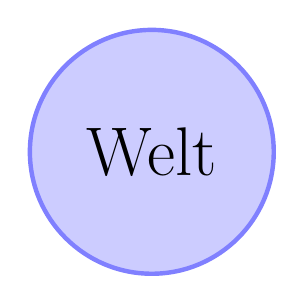
\begin{tikzpicture}
    \node[circle,fill=blue!20,draw=blue!50,ultra thick,inner sep=.5cm] {\Huge{Welt}};
  \end{tikzpicture}
}

\only<2>{
  \begin{tikzpicture}
  \node[circle,fill=blue!20,draw=blue!50,ultra thick,text width=1.5cm,align=center] (northAmerica) {Nord Amerika};
  \node[circle,fill=blue!20,draw=blue!50,ultra thick,text width=1.5cm,align=center] (southAmerica)[below=1mm of northAmerica] {Süd Amerika};
  \node[circle,fill=blue!20,draw=blue!50,ultra thick] (Europa) [right=1cm of northAmerica] {Europa};
  \node[circle,fill=blue!20,draw=blue!50,ultra thick] (Afrika)[below=5mm of Europa] {Afrika};
  \node[circle,fill=blue!20,draw=blue!50,ultra thick] (Asien) [right=1mm of Europa] {Asien};
  \node[circle,fill=blue!20,draw=blue!50,ultra thick] (Australien) [right=1cm of Afrika,yshift=-5mm] {Australien};
  \end{tikzpicture}
}
  \end{center}
}


%%% Local Variables: 
%%% mode: latex
%%% TeX-master: "main"
%%% End: 
